The analytic calculations of \citet{Jones2001} are based on the wobble angle 
$\wobbleangle$ which the spin-vector makes with the axis about which it precesses.
This axis depends on the mass distribution, and any applied torques. Before
continuing we discuss what this wobble angle is given by in different cases.

To understand the wobble angle we refer to figure \ref{fig: reference plane}
illustrating the so-called reference plane from \citet{Jones2001}
\begin{figure}
    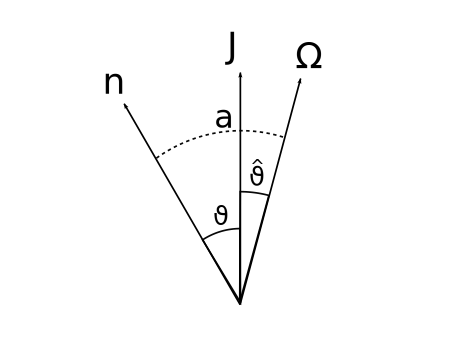
\includegraphics[width=0.2\textwidth]{/home/greg/Neutron_star_modelling/Illustrations/ReferencePlane/ReferencePlane.pdf}
    \caption{The reference plane containing the angular momentum vector $\spin$,
    the angular momentum vector $\L$ and the symmetry axis $n$ lying along the
    body-frame $\z$ axis. The dotted line indicates the polar angle $a$ between
    the body-frame $\z$ axis and the spin vector.}
    \label{fig: reference plane}
\end{figure}
This reference plane is a direct result of the relation 
\begin{align}
    L_{a} = I_{ab} \omega_{b} &&& I_{ab} = I_{0} \delta_{ab} + \epsI\delta_{3a}\delta_{3b}
\end{align}
since $\mathbf{n}$ lies along the $\z$ axis of the body frame. It was shown by
\citet{Jones2001} that for nearly spherical bodies
\begin{equation}
    \hat{\theta} \approx \epsI \sin\theta \cos\theta.
\end{equation}
Taking also the limit that $\theta \ll 1$ it can be shown that
\begin{equation}
    \hat{\theta} \approx \epsI \theta
\end{equation}
and so when comparing the two angles $\hat{\theta} \ll \theta$ such that 
$a\approx \theta$.

For a biaxial body free of torques, the spin vector precesses about the
symmetry axis of the moment of inertia $\mathbf{n}$. Using the approximations
mentioned above then the wobble angle is given by
\begin{equation}
    \wobbleangle \approx \theta.
\end{equation}
Therefore, solutions without precession correspond to $a=0$.
%For triaxial bodies it can precess
%about either of the stable axis of the moment of inertia \citep{Landau1969}. 

Including the EM torque from equation \eqref{eqn: torque} introduces two effects:
the first and the largest is the transformation induced by the anomalous torque
which causes the spin-vector to precess about the principle axis of an
\emph{effective} body-frame. This has already been discussed in chapter \ref{sec:
effective body frame} and results in a wobble angle
\begin{equation}
    \wobbleangle \approx \theta - \beta
    \label{eqn: wobble angle no SD}
\end{equation}
where $\beta$ is the rotation from the body-frame to the effective body-frame.
In this case non-precessing solutions correspond to $a \approx \beta$.

The second, smaller effect is that, even without the anomalous torque the spin-down 
torque introduces a time-varying component to the angular momentum vector. Which
will change the axis of precession. The magnitude of this time
varying component is given by 
\begin{equation}
|\dot{\L}| \sim L \omega \hat{\theta}
\end{equation} 
this can be equated to the magnitude of the spindown torque
\begin{equation}
|T_{\mathrm{sd}}| = I_{0}|\dot{\spin}|
\end{equation}
rearranging for the angle between the spin-vector and angular momentum yeilds
\begin{equation}
    \hat{\theta} = \frac{I_{0}\dot{\omega}}{I \omega^{2}} = \frac{P}{\tauS}
\end{equation}
The wobble angle due to this spin-down torque is then given by 
\begin{align}
    \wobbleangle_{\mathrm{SD}} & = \theta + \hat{\theta}\\
                 & = \hat{\theta}\left(1 + \frac{1}{\epsI}\right) \\
                 & = \frac{P}{\tauS}\left(1 + \frac{1}{\epsI}\right) \\
                 & \approx \frac{P}{\tauS}{\frac{1}{\epsI}}
    \label{eqn: spindown wobble angle}
\end{align}
Therefore we can write the wobble angle in general as
\begin{equation}
    \wobbleangle = \theta - \beta + \frac{P}{\tauS}\frac{1}{\epsI}
    \label{eqn: wobble angle}
\end{equation}
Now for solutions where the precession is important the final term
will be negligable and so we generally refer to equation \eqref{eqn: wobble angle no SD}.
However, when we set up initial conditions to minimise the precession: either
$a_{0}=0$ for free precession or $a_{0} = \beta$ when incuding the anomalous
torque; the approximations we made earlier become important. Now the wobble angle
due to the spindown can dominate and so we should use the full expression in
equation \eqref{eqn: wobble angle}.
